\documentclass[10pt]{article}
\usepackage{amsmath,
            bm,
            xstring,
            upgreek,
            graphicx,
            booktabs,
            enumitem,
            booktabs,
            subcaption,
            tcolorbox,
            newfloat,
            graphicx,
            tocloft}
\usepackage[hang,flushmargin]{footmisc}
\usepackage[margin=2cm]{geometry}
\usepackage[colorlinks,linkcolor=blue,citecolor=purple]{hyperref}
\usepackage[backend=bibtex,citestyle=numeric,sorting=none,
            maxcitenames=2,isbn=false,url=false]{biblatex}
% --------------------------------------------------------------------------------------------------
% paths
\graphicspath{
  {figs/}
  {figs/tikz/}
  {../../outputs/figs/plots/compare/}
  {../../outputs/figs/2d/}}
\usepackage{tikz}
\usepackage{tikz-qtree}
\usetikzlibrary{positioning,arrows.meta,quotes,calc}
\tikzset{%
  arrow/.style    = { ->, >=Latex,  line width = 0.4mm, rounded corners, draw = black, every edge/.style={arrow} },
  arrow/.style    = { ->, >=Latex,  very thick, rounded corners,
                      fill = #1, draw = #1 },
  tbox/.style     = { fill = #1!20!white, draw = #1!80!white, thick, align = center,
                      minimum width = 0.8cm, minimum height = 0.6cm, node distance = 1.5cm },
  leaf/.style     = { fill = #1!20!white, draw = #1!80!white, thick, align = center, rounded corners = 0.3cm, grow = down,
                      minimum width = 1.2cm, minimum height = 0.6cm, node distance = 1.5cm }
}
\newcommand{\connectall}[2]{
  \foreach \s in {#1} {
    \foreach \t in {#2} {
      \draw[arrow,<->] (\s) -- (\t);
    }
  }
}
\addbibresource{../../refs/refs.bib}
\usepackage{hyperref,catchfile,ifplatform,xstring}

% Try to load the most recent commit key from the local .git files
% so that the compiled appendix references the "current" version
% and not one in the future, where things may have changed.
% As usual, windows breaks something.

% online repos
\newcommand{\projrepo}{https://github.com/c-uhs/turnover}
\newcommand{\epimodelrepo}{https://github.com/c-uhs/epi-model}

% commit keys

\ifwindows
  \newcommand{\projcommit}{master}
\else
  \newcommand{\projcommitfile}{../../.git/refs/heads/master}
  \CatchFileDef{\projcommit}{\projcommitfile}{\endlinechar=-1}
\fi
\newcommand{\epimodelcommit}{master}

% some handy pre-formatted links
\newcommand{\projrepocommit}{\href{\projrepo/tree/\projcommit}{\texttt{\projrepo}}}
\newcommand{\epimodelrepocommit}{\href{\epimodelrepo/tree/\epimodelcommit}{\texttt{\epimodelrepo}}}

% create box float
\newtcolorbox{fboxed}{sharp corners = all, colback = white!97!black, boxrule=1pt}
\DeclareFloatingEnvironment[name=Box]{floatbox}
% lengths
\setlength{\skip\footins}{24pt}
\setlength{\abovecaptionskip}{6pt}
\setlength{\belowcaptionskip}{6pt}
\setlength{\cftbeforesecskip}{8pt}
\setlength{\parindent}{0pt}
\setlength{\parskip}{6pt}
\setlength{\tabcolsep}{4pt}
\setlength{\footnotemargin}{8pt}
\newlength{\figi}  \setlength{\figi}  {0.800\textwidth}
\newlength{\figii} \setlength{\figii} {0.490\textwidth}
\newlength{\figiii}\setlength{\figiii}{0.325\textwidth}
% numbering & bullets
\setlist[itemize]{label=\raisebox{0.2em}{\footnotesize\textbullet},topsep=0pt,itemsep=0pt}
\setlist[enumerate,1]{label=\arabic*.}
\setlist[enumerate,2]{label*=\arabic*.}
\numberwithin{equation}{section}
% shorthands
\renewcommand{\zeta}{\upzeta}
\newcommand{\N}{{\mbox{\footnotesize{\textit{N}}}}}
\newcommand{\G}{{\mbox{\footnotesize{\textit{G}}}}}
\newcommand{\tarr}[1]{{\def\arraycolsep{3pt}[\begin{matrix}\StrSubstitute{#1}{,}{&}\end{matrix}]}}
\newcommand{\hreftt}[1]{\href{#1}{\texttt{#1}}}
% references
\newcommand{\citet}[1]{\citeauthor{#1}~(\citeyear{#1})~\cite{#1}}
\newcommand{\eq}[1]{Eq.~(\ref{#1})}
\newcommand{\fig}[1]{Figure~\ref{#1}}
\newcommand{\tab}[1]{Table~\ref{#1}}
\newcommand{\app}[1]{Appendix~\ref{#1}~\nameref{#1}}
% --------------------------------------------------------------------------------------------------
\title{On Parameterizing Risk Group Dynamics in Simulated STI Epidemics}
\author{Jesse Knight, Linwei Wang, Huiting Ma, Sharmistha Mishra}
%%%%%%%%%%%%%%%%%%%%%%%%%%%%%%%%%%%%%%%%%%%%%%%%%%%%%%%%%%%%%%%%%%%%%%%%%%%%%%%%%%%%%%%%%%%%%%%%%%%%
%%%%%%%%%%%%%%%%%%%%%%%%%%%%%%%%%%%%%%%%%%%%%%%%%%%%%%%%%%%%%%%%%%%%%%%%%%%%%%%%%%%%%%%%%%%%%%%%%%%%
%%%%%%%%%%%%%%%%%%%%%%%%%%%%%%%%%%%%%%%%%%%%%%%%%%%%%%%%%%%%%%%%%%%%%%%%%%%%%%%%%%%%%%%%%%%%%%%%%%%%
\begin{document}
%%%%%%%%%%%%%%%%%%%%%%%%%%%%%%%%%%%%%%%%%%%%%%%%%%%%%%%%%%%%%%%%%%%%%%%%%%%%%%%%%%%%%%%%%%%%%%%%%%%%
\maketitle
\tableofcontents
\subsection*{Key Contributions}
\begin{enumerate}
  \item Formalize a mathematical framework for risk group demographics
  \item Describe methods for deriving risk group demographic parameters from common data sources
  \item Illustrate differences in modelled projections
  for different implementations of risk group demographics,
  using an example sexually transmitted infection
\end{enumerate}
\clearpage
%%%%%%%%%%%%%%%%%%%%%%%%%%%%%%%%%%%%%%%%%%%%%%%%%%%%%%%%%%%%%%%%%%%%%%%%%%%%%%%%%%%%%%%%%%%%%%%%%%%%
\section{Introduction}\label{s:intro}
Core group theory has long underpinned modelling of STI epidemics.
It generally describes maintenance of an epidemic by
high levels of exposure in a small subset of individuals,
relative to a larger general population with less exposure~\cite{Yorke1978}.
When considering one or more core groups
-- i.e.\ a population composed of several risk-stratified groups --
the epidemic characteristics are known to depend on
the group sizes, relative exposures, and rates of sexual mixing between groups.
Less discussed is a similar dependence on
movement of individuals between risk groups, which we call ``turnover''.%
\footnote{In early works, such as \cite{Stigum1994},
  movement of individuals between risk groups is often called ``migration'';
  in order to avoid confusion with population entry / exit,
  we prefer the term ``turnover''.}
This turnover of individuals between risk groups has a similar effect to
sexual mixing between groups, making it
an important feature to include in representative models~\cite{Stigum1994}.
\par
Models with more than two risk groups
are increasingly relevant for exploring epidemic nuance
and for aligning model outputs with programmatic decision support
-- i.e.\ prioritization specific interventions for specific risk groups. % \cite{?}
Yet, implementations of risk groups and turnover in recent models vary widely,
from no modelled risk groups~\cite{Estill2012,Barnighausen2012}
to seven risk groups with highly context-specific turnover [[best Mishra 7-groups citation]].
In fact, many HIV models still do not consider turnover,
despite the fact that rates of movement between risk groups
can play an important role during estimation of intervention impact
following model fitting to calibration targets~\cite{Eaton2014}.
\par
Two major challenges exist to implementing turnover,
which may help explain its inconsistent usage.
First, unlike behavioural parameters,
estimating the rates of movement between groups
directly from cross-sectional survey data is difficult,
and typically requires strong assumptions.
Second, ensuring the relative sizes of risk groups do not vary
dramatically over time requires
careful selection rates of turnover among groups,
or other compensatory parameters.
Prior works have generally solved this problem \textit{ad hoc},
without providing a generalized approach,
while some simply rely on a ``burn-in'' period,
which permits equilibriation of risk group sizes due to turnover dynamics
before introduction of the infection.
\par
We therefore expect that a unified framework for
defining and parameterizing risk group dynamics
would be of great use.
We present such a framework here,
and draw direct links to modelling assumptions and relevant sources of data.
Building on previous work by~\citet{Stigum1994},
we then leverage this framework to explore the impact of
several risk group implementations on model outputs (incidence, prevalence)
in a representative model.
%%%%%%%%%%%%%%%%%%%%%%%%%%%%%%%%%%%%%%%%%%%%%%%%%%%%%%%%%%%%%%%%%%%%%%%%%%%%%%%%%%%%%%%%%%%%%%%%%%%%
\section{The System}\label{s:system}
This section introduces a system of compartments, flows between them, and equations
which can be used to describe risk group dynamics.
\par
We denote the variable representing
the size of risk group $i \in [1, \dots, \G]$ as $x_i$
and the vector of all $x_i$ as $\bm{x}$.
The total population size is denoted $\N = \sum_i x_i$,%
\footnote{In many models, ``total population'' actually refers to
  an age-constrained range.}
and the proportions represented by each group by $\hat{x}_i = x_i \N^{-1}$.
The rate of population entry for all groups is denoted by $\nu$, and
the rate of exit by $\mu$.
We do not consider disease-attributable death, which may vary by group,
though this will be the subject of future work.
All rates have units \textit{per year} ($\mathrm{yr}^{-1}$).
The proportion of the entering population who are in group $i$,
which may not be equal to the proportion of the current population in group $i$,
is denoted $\hat{e}_i$.
Since the rate of entry $\nu$ is typically expressed as
a proportion of the total population size $\N$,%
we model the theoretical entering population $\bm{e}$ as also having size $\N$,
so that $e_i = \hat{e}_i \N$.
\par
Turnover transitions can occur between any two groups, in either direction;
therefore we denote the turnover rates as a $\G \times \G$ matrix $\zeta$,
where $\zeta_{ij}$ corresponds to the transition $x_i \rightarrow x_j$.
An explicit definition is given in Eq.~(\ref{eq:zeta}),
where the diagonal elements are denoted $*$ since they represent
transitions from a group to itself, which is inconsequential.
\begin{equation}\label{eq:zeta}
\zeta = \left[\begin{array}{cccc}
         *           & x_1  \rightarrow x_2 & \cdots & x_1 \rightarrow x_\G \\[0.5em]
x_2  \rightarrow x_1 &          *           & \cdots & x_2 \rightarrow x_\G \\[0.5em]
      \vdots         &       \vdots         & \ddots &       \vdots         \\[0.5em]
x_\G \rightarrow x_1 & x_\G \rightarrow x_2 & \cdots &          *
\end{array}\right]
\end{equation}
These transition flows and the associated rates
are summarized for $\G = 3$ in \fig{fig:system}.
\begin{figure}[h]
  \centering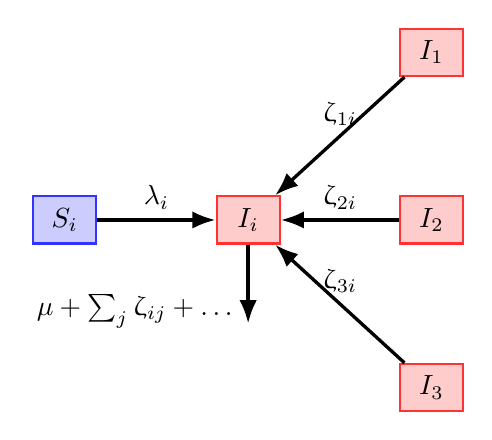
\begin{tikzpicture}
  \node(y)[tbox=red] {$I_i$};
  \node(s)[tbox=blue, left = of y]{$S_i$};
  \node(b)[tbox=red, right = of y]{$I_2$};
  \node(a)[tbox=red, above = of b]{$I_1$};
  \node(c)[tbox=red, below = of b]{$I_3$};
  \node(x)[below = of y]{};
  \draw[arrow,<-] (y) -- node[above] {$\lambda_{i}$} (s);
  \draw[arrow,<-] (y) -- node[above] {$\zeta_{1i}$} (a);
  \draw[arrow,<-] (y) -- node[above] {$\zeta_{2i}$} (b);
  \draw[arrow,<-] (y) -- node[above] {$\zeta_{3i}$} (c);
  \draw[arrow,->] (y) -- node[below left] {$\mu + \sum_j{\zeta_{ij}} + \dots$} (x);
\end{tikzpicture}
  \caption{System of compartments and flows between them for $\G = 3$}
  \label{fig:system}
\end{figure}
%\par
%Some key assumptions of this work:
%\begin{itemize}
%  \item The health states of individuals moving between risk groups due to turnover
%  is proportional to the health states of the group overall.
%  \item Disease-attributable death has negligible impact on risk-group proportions.
%  \item 
%\end{itemize}
% ==================================================================================================
\subsection{Parameterization}\label{ss:params}
Next, we explore methods for estimating the values of parameters
in the system described above
($\nu$, $\mu$, $\bm{\hat{x}}$, $\bm{\hat{e}}$, and $\zeta$)
directly from some commonly available sources of data.
\par
In most cases, there will not be sufficient data to directly estimate all parameters,
especially $\zeta$.
The next section outlines additional methods to solve for these values.
% * (is this true anymore?)
% * (discuss latent assumptions with each of these approaches)
% --------------------------------------------------------------------------------------------------
\subsubsection{Total Population Size}\label{sss:params-nu-mu}
%\begin{table}
%  \centering
%  \caption{Methods for deriving entry $\nu$ and exit $\mu$ rates}
%  \label{tab:nu-mu}
%  \begin{tabular}{lclll}
	\toprule
	Parameter       &    Symbol    & Data Sources & Key Equations & Validation \\
	\midrule
	Population Size &   $\N(t)$    &              &               &            \\
	Growth rate     & $\growth(t)$ &              &               &            \\
	Entry rate      &   $\nu(t)$   &              &               &            \\
	Exit rate       &   $\mu(t)$   &              &               &            \\
	\bottomrule
\end{tabular}
%\end{table}
The model of total population size over time is defined by
entry and exit rates, $\nu$ and $\mu$, as in:
\begin{subequations}
  \begin{align}
  \N(t) &= \N_0 {\big(1+\mathcal{G}(t)\big)}^{t} \label{eq:growth-N}\\
  \mathcal{G}(t) &= \nu(t) - \mu(t)              \label{eq:growth-G}
  \end{align}
\end{subequations}
and we note that the average duration of an individual in the model at time $t$
is given by:
\begin{equation} \label{eq:duration-model}
  \delta(t) = \mu^{-1}(t)
\end{equation}
Variation in rate of entry across risk groups is captured in $\bm{\hat{e}}$,
and we generally do not stratify rate of exit by activity group
(besides disease-attributable death);
therefore, we can assume that $\nu$ and $\mu$ do not vary across risk groups,
which allows us to derive them with $\N(t)$, independent of
the population proportions $\bm{\hat{x}}$, $\bm{\hat{e}}$, and turnover $\zeta$.
\par
The simplest approach assumes a constant population size $\N(t) = \N_0$,
or a growth rate of zero, yielding $\nu = \mu$.
However, this does not reflect the true positive population growth of most contexts,
and may result in underestimated incidence,
due to the relative reduction in inflow of susceptible individuals.
% verified in code, see:
% https://github.com/c-uhs/turnover/blob/f029bd1/outputs/figs/debug/incidence-nu.gif
\par
Another approach is to fix $\mathcal{G}(t)$ as some constant.
When using this approach, extra care should be taken to ensure
the resulting $\N(t)$ matches any available population size estimates to a reasonable degree.
\par
Typically, data will be available for the total size of the population over time $\N(t)$,
so the growth rate for each time interval $t_i$
can be derived by rearranging \eq{eq:growth-N}:
\begin{equation}
\mathcal{G}(t_i) = {\left(\frac{\N(t_{i+1})}{\N(t_{i})}\right)}^{-(t_{i+1}-t_i)} - 1
\end{equation}
All of these approaches help define $\mathcal{G}(t)$, but leave one degree of freedom,
since any choice of $\mu(t)$ can be compensated by $\nu(t)$ to yield the desired $\mathcal{G}(t)$.
However, we can usually leverage the known duration of individuals in the model $\delta(t)$
to choose $\mu(t)$ as in \eq{eq:duration-model}.
This can come from an assumed duration of sexual activity,
or a constant, predefined age range relevant to parameterization.
Then, we can solve for $\nu(t)$ using \eq{eq:growth-G}.
% --------------------------------------------------------------------------------------------------
\subsubsection{Turnover}\label{sss:params-turnover}
% TODO: discuss common approaches - especially turnover is constant, or zero.
% TODO: discuss more the assumptions throughout.
Next, we assume that $\nu(t)$ and $\mu(t)$ are known,
and we focus on resolving $\bm{\hat{e}}(t)$ and $\zeta(t)$.
Similar to above, we will first formulate the problem as a system of equations;
then we will consider which data and assumptions we can leverage to solve the system.
\par
We begin by defining the ``conservation of mass'' equation for a given group $x_i$,
where that the rate of change of the group
is simply the sum of flows in~/~out of the group:
\begin{equation}\label{eq:mass-balance}
\frac{d}{dt}x_i
= \nu \thinspace e_i + \sum_{j}{\zeta_{ji} \thinspace x_j}
- \mu \thinspace x_i - \sum_{j}{\zeta_{ij} \thinspace x_i}
\end{equation}
While \eq{eq:mass-balance} is written in terms of
absolute population sizes $\bm{x}$ and $\bm{e}$,
it is equivalent to divide through by $\N$, yielding a system in terms of
proportions $\bm{\hat{x}}$ and $\bm{\hat{e}}$,
which is often more useful, since $\N$ need not be known.
\par
We further assume that the average proportions of each group $\hat{x}_i$ do not change over time.
Therefore, the desired rate of change for risk group $i$
will be equal to the growth of the risk group, $\mathcal{G} x_i$.
Substituting this into \eq{eq:mass-balance},
and simplifying, we have:
\begin{equation}\label{eq:system}
\nu \thinspace x_i
= \nu \thinspace e_i + \sum_{j}{\zeta_{ji} \thinspace x_j}
- \sum_{j}{\zeta_{ij} \thinspace x_i}
\end{equation}
Now, depending on the number of risk groups, we have
$\G$ and $\G(\G-1)$ unknowns in $\bm{e}$ and $\zeta$, totalling $\G^2$ variables to resolve.
We denote these variables as the vector $\bm{\theta} = \left[\bm{e}, \bm{z}\right]$,
where $\bm{z} = \mathrm{vec}_{i \ne j}(\zeta)$;
this allows us to define
a system of linear equations of the form:
\begin{equation}\label{eq:system-matrix}
\bm{b} = A \thinspace \bm{\theta}
\end{equation}
where $A$ is a $\G \times \G^2 $ matrix
and $\bm{b}$ is a $\G$-length vector,
representing the right-hand side and left-hand side of \eq{eq:system}, respectively.
In this form, we can use $A^{-1}\bm{b} = \bm{\theta}$ to solve for $\bm{\theta}$.
\par
Unfortunately, for any $\G > 1$, the system is underdetermined by a factor of $\G(\G-1)$,
meaning there are many combinations of $\bm{e}$ and $\zeta$ which satisfy \eq{eq:system}.
Therefore, we now resume our task of leveraging data and assumptions
to define a unique solution.
\par
Our first tool is another equation.
We note that the duration of time spent in a particular group $\delta_i$
is the inverse of all efferent flow rates:
\begin{equation}\label{eq:duration-group}
\delta_i = {\bigg(\mu + \sum_{j}{\zeta_{ij}}\bigg)}^{-1}
\end{equation}
These durations could be derived from survey data, including for key populations,
or they could be assumed.
Rearranging \eq{eq:duration-group}, we obtain
${\delta_i}^{-1} - \mu = \sum_{j}{\zeta_{ij}}$,
which yields an additional $\G$ equations in our linear system -- i.e.\ rows of $A$ and $\bm{b}$.
For $\G = 2$, this provides enough constraints to fully determine the system,
as shown in \app{a:example-systems},
but for larger $\G$, still more constraints are needed.
\par
The simplest additional constraints can be elements in $\bm{\theta}$ which are directly specified
-- i.e.\ elements of of $\bm{e}$ or $\zeta$.
For example, the proportion of individuals who
move from one risk group to another each year ($\zeta_{ij}$)
may be assumed or derived from data.
Similarly, the distribution of individuals
across risk groups in the entering population $\bm{\hat{e}}$
may be approximated using the proportions among
the lowest age group for which data are available.
In each case, the value specified is appended to $\bm{b}$,
and a row appended to $A$ of the form: $[0,\dots,1,\dots,0]$,
with $1$ in the position of the element in $\bm{\theta}$.
\par
There are, however, two notable caveats to this approach.
First, not all combinations of specified elements will add an equal number of constraints.
Specifying all elements of $\bm{e}$
will only add $\G-1$ (not $\G$) constraints,
since $\sum \bm{\hat{e}} = 1$, so the final element adds no new information.
Similarly, specifying all elements of $\zeta_{ij}$ for a given $i$
as well as the duration for the group $\delta_i$
will only add $\G-1$ (not $\G$) constraints,
since \eq{eq:duration-group} must hold.
%\footnote{Recall that the diagonal elements of $\zeta$ are inconsequential,
%  so only $\G-1$ elements of $\zeta_{ij}$ may be specified at all for a given $i$.}
Second, not all combinations of specified values will yield a valid solution,%
\footnote{Even rank-deficient systems be inconsistent.}
and it is unfortunately difficult to anticipate problematic combinations.
\par
Finally, we note that additional constraints may be avoided altogether if we pose the problem
as an optimization problem, namely:
\begin{equation}\label{eq:system-optimize}
\bm{\theta}^{*} = {\arg \min}
  \thinspace f(\bm{\theta}),
  \quad \textrm{subject to:}
  \enspace\bm{b} = A\thinspace\bm{\theta};
  \enspace\bm{\theta} \ge 0
\end{equation}
where $f$ is a function such as ${\left|\left| \thinspace\cdot\thinspace \right|\right|}_2$.
However, the choice of $f$ implies a prior on the values of $\bm{\theta}$,
and so introduces bias in the solution.
% ==================================================================================================
\subsection{Previous Approaches}
%In this section, we will examine previous approaches to modelling
%risk groups in simulated HIV epidemics,
%and the assumptions inherent to these methods.
%Box~\ref{box:assumptions} summarizes
%the most common assumptions regarding the dynamics of these risk groups,
%while \tab{tab:prior-work} summarizes previous works
%with respect to these assumptions.
%\par
%Many of the previously proposed models of HIV transmission
%follow Assumption~\ref{ass:risk-groups-no} and do not consider heterogeneity
%in risk of acquisition within major demographic groups,
%such as heterosexual men / women, and MSM.
%This is a significant assumption,
%and may lead to large discrepancies with models which do consider risk heterogeneity,
%as explored in Section~\ref{s:exp}.
%Moreover, this assumption precludes any consideration of turnover,
%since there is only one risk group, $\G = 1$.
%\par
%* (discussion of each assumption in turn)
\begin{floatbox}
  \caption{Common assumptions regarding the dynamics of risk groups}
  \label{box:assumptions}
  \begin{fboxed}
  \begin{enumerate}[leftmargin=1em]
    \item\label{ass:risk-groups}\textbf{Risk Groups:}
    Populations are stratified by risk of infection acquisition.
    \begin{enumerate}
      \item\label{ass:risk-groups-no}\textbf{No:} $G = 1$;
      Populations are homogeneous in risk of infection acquisition.
      \item\label{ass:risk-groups-yes}\textbf{Yes:} $G > 1$;
      Heterogeneity in risk of infection acquisition within populations is considered.
    \end{enumerate}
    \item\label{ass:turnover}\textbf{Turnover:}
    Individuals may move between risk groups.
    \begin{enumerate}
      \item\textbf{No:} $\zeta = 0$;
      Individuals do not move between risk groups.
      \item\textbf{Constant:} $\zeta > 0$;
      Individuals move between risk groups at a constant rate.
%      \item\textbf{Dynamic:} $\zeta = f$;
%      Individuals move between risk groups in dynamically.
    \end{enumerate}
    \item\label{ass:pop-growth}\textbf{Population Growth:}
    Increase in the total $N$ over time.
    \begin{enumerate}
      \item\textbf{No:} $\nu = \mu$;
      Population size $N$ is constant.
      \item\textbf{Yes:} $\nu > \mu$;
      Population size $N$ increases, at some constant or data-driven rate.
    \end{enumerate}
  \end{enumerate}
\end{fboxed}

\end{floatbox}
\begin{table}
  \centering
  \caption{Summary of prior work with respect to modelled risk group dynamics.}
  \label{tab:prior-work}
  \input{tabs/tab-prior-work.tex}
\end{table}
\clearpage
%%%%%%%%%%%%%%%%%%%%%%%%%%%%%%%%%%%%%%%%%%%%%%%%%%%%%%%%%%%%%%%%%%%%%%%%%%%%%%%%%%%%%%%%%%%%%%%%%%%%
\section{Experiment}\label{s:exp}
We have described an approach to parameterizing models of risk group dynamics
which hopefully highlights the
\textit{feasibility} of including such model components based on available data.
Next, we will explore the
\textit{importance} of including these components
through comparison of projected model outputs
across different implementations of risk group dynamics.
Specifically, we will compare structural variants
involving differences in population growth, number of risk groups, and turnover.
% ==================================================================================================
\subsection{Model \& Simulations}\label{ss:model}
We start with a simple deterministic model of heterosexual HIV transmission,
which is meant to be generally representative of a plausible HIV epidemic,
rather than any specific context.
The model includes three health states:
susceptible~$\mathcal{S}$, infected~$\mathcal{I}$, and on treatment~$\mathcal{T}$,
as shown in \fig{fig:health-states},
and $\G = 3$ levels of sexual activity (risk groups):
high~$H$, medium~$M$, and low~$L$.
Individuals of sex $\mathit{k}$ in risk group $i$ are assumed to
form sexual partnerships at a rate $C_{ki}$
with individuals of the opposite sex $\mathrm{k}$.
The probability of partnership formation with
a partner of sex $\mathrm{k}$ in risk group $\mathrm{i}$
is assumed to follow
the formulation proposed by \citeauthor{Garnett1994}~\cite{Garnett1994}: % \cite{?} someone else proposed this first ...
\begin{equation}
  \rho_{\mathit{ki}\mathrm{ki}} =
  (1-\epsilon)\psi_{\mathit{ki}\mathrm{ki}}
   +(\epsilon)\pi_{\mathit{ki}\mathrm{ki}}
\end{equation}
where $\epsilon$ is a parameter controlling the dominance of
assortative $\psi$ ($\epsilon = 0$) or proportional $\pi$ ($\epsilon = 1$) mixing.
\begin{figure}
  \centering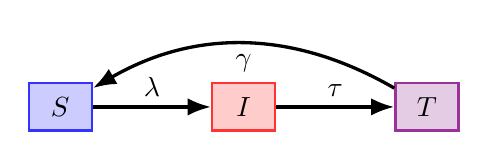
\begin{tikzpicture}
\node(S) [tbox=blue] at (0.0,0.0)   {$S$};
\node(I) [tbox=red,    right = of S]{$I$};
\node(T) [tbox=violet, right = of I]{$T$};

\draw[arrow=black] (S) edge["$\lambda$"] (I);
\draw[arrow=black] (I) edge["$\tau$"]  (T);
\draw[arrow=black] (T) edge["$\gamma$", bend right] (S);
\end{tikzpicture}
  \caption{Modelled health states}\label{fig:health-states}
\end{figure}
\par
Transmission of HIV from infected $\mathcal{I}$ to susceptible $\mathcal{S}$ individuals
is assumed to occur with probability $\beta_{\mathit{k}\mathrm{k}}$ per partnership.
Individuals on treatment $\mathcal{T}$ are not considered infectious.
The force of infection for susceptible individuals of sex $k$ in risk group $i$
is therefore modelled using the following equation:%~\cite{?}
\begin{equation}
  \lambda_{ki} =
  C_{\mathit{ki}}
  \sum_{\mathrm{ki}}
  \rho_{\mathit{ki}\mathrm{ki}} \thinspace
  \beta_{\mathit{k}\mathrm{k}}
  \frac{\mathcal{I}_{\mathrm{ki}}}{\N_{\mathrm{ki}}}
  \label{eq:foi}
\end{equation}
Infected individuals are assumed to be diagnosed and begin treatment at a rate $\tau$ (per year).
As described in Section \ref{s:system},
individuals enter the model at a rate $\nu$,
exit at a rate $\mu$,
and transition from risk group $i$ to group $j$ at a rate $\zeta_{ij}$.
The default parameters for this base model are summarized in
\tab{tab:params-base}.
\begin{table}[b]
  \centering\caption{Base model parameters. All rates have units $\mathrm{year}^{-1}$ and durations are in $\mathrm{years}$.}
  \label{tab:params-base}
  \begin{tabular}{clc}
	\toprule
	    Symbol     & Description                                                                                             &         Value         \\
	\midrule
	   $\beta$     & transmission probability per partnership: men $\rightarrow$ women, women $\rightarrow$ men              &    \tarr{0.1,0.05}    \\
	  $\epsilon$   & mixing parameter where: 1 $\rightarrow$ proportional and 0 $\rightarrow$ assortative \cite{Garnett1994} &          1.0          \\
	    $\tau$     & rate of treatment initiation among infected                                                             &          0.1          \\
	    $\N_0$     & initial population size                                                                                 &         1000          \\
	\midrule
	$\bm{\hat{x}}$ & proportion of system individuals: high, medium, low activity                                            & \tarr{0.04,0.20,0.76} \\
	$\bm{\hat{e}}$ & proportion of entering individuals: high, medium, low activity                                          & \tarr{0.04,0.20,0.76} \\
	$\bm{\delta}$  & average duration spent in: high, medium, and low activity groups                                        &    \tarr{5,15,25}     \\
	     $C$       & rate of partner change among individuals: high, medium, low activity                                    &     \tarr{25,5,1}     \\
	    $\nu$      & rate of population entry                                                                                &         0.05          \\
	    $\mu$      & rate of population exit                                                                                 &         0.03          \\
	\bottomrule
\end{tabular}
\end{table}
\par
Using this model (and variants, described below),
simulated epidemics are initialized at $t = 0$ with $\N_0 = 1000$ individuals,
distributed proportionally according to $\bm{\hat{x}}$.
Among these individuals, 6 are infected, and the remainder are susceptible;
for $\G = 3$, this corresponds to one infected person in each sex-risk group,
while for $\G = 1$, this corresponds to three infected people in each sex.
Simulated epidemics are solved numerically using Euler's method
with a time step of $dt = 0.1$ years.
% ==================================================================================================
\subsection{Model Variants}\label{ss:exp-variants}
Drawing on the most common assumptions outlined in Box~\ref{box:assumptions},
we define a series of six structural model variants (V1~--~V6) for investigation.
These variants, summarized in \fig{fig:variant-tree}, include
zero versus nonzero population growth ($\nu = \mu$ vs $\nu > \mu$),
homogeneous versus heterogeneous risk ($\G = 1$ vs $\G = 3$),
and zero versus nonzero turnover among risk groups ($\zeta = 0$ vs $\zeta > 0$).
\begin{figure}
  \centering\newlength{\lvl}\setlength{\lvl}{1cm}
\newcounter{variant}
\newcommand{\nvar}{\stepcounter{variant}V\thevariant}
\begin{tikzpicture}[
    level distance = \lvl,
    sibling distance = 0.3\lvl,
    every path/.append style = { thick },
    edge from parent path = {
      (\tikzparentnode) -- +(0.0,-0.5\lvl) -| (\tikzchildnode)
    },
    frontier/.style = { distance from root = 4\lvl }
  ]
  \Tree
    [.{}
      [.\node[branch]{$\nu>\mu$};
        [.\node[branch]{$\G=3$};
          [.\node[branch]{$\zeta > 0$}; \node[leaf]{\nvar}; ]
          [.\node[branch]{$\zeta = 0$}; \node[leaf]{\nvar}; ]
        ]
        [.\node[branch]{$\G=1$}; \node[leaf]{\nvar}; ]
      ]
      [.\node[branch]{$\nu=\mu$};
        [.\node[branch]{$\G=3$};
          [.\node[branch]{$\zeta > 0$}; \node[leaf]{\nvar}; ]
          [.\node[branch]{$\zeta = 0$}; \node[leaf]{\nvar}; ]
        ]
        [.\node[branch]{$\G=1$}; \node[leaf]{\nvar}; ]
      ]
    ]
\end{tikzpicture}

  \caption{Summary of 6 structural model variants with respect to simulated risk group dynamics.
    $\nu$:~rate of population entry,
    $\mu$:~rate of population exit,
    $\G$:~number of risk groups,
    $\zeta$:~rates of population turnover}
  \label{fig:variant-tree}
\end{figure}
\par
In order to facilitate fair comparisons across model variants with respect to parameter values,
we start from the base model described above (V1~in \fig{fig:variant-tree}),
and aim to make simplifications with minimal impact on system characteristics.
% not sure how to communicate this idea...
For example, when moving from $\nu > \mu$ to $\nu = \mu$,
we ensure the average duration of individuals in the model $\mu^{-1}$ is unchanged
by fixing $\mu$ and reducing $\nu$ to match (V4~--~V6).
Similarly, when collapsing the stratification of risk groups from $\G = 3$ to $\G = 1$ (V3,~V6),
we define the homogeneous partner change rate $C$
as the weighted average of the previously risk-stratified $C$.
Finally, considering rates of turnover $\zeta$
(which are only applicable for V1,~V4)
we fully determine the system, as outlined in Section~\ref{sss:params-turnover},
by specifying the average duration of individuals in each group $\bm{\delta}$,
as well as the distribution of individuals entering the model $\bm{\hat{e}}$,
and the proportion of high activity individuals moving to the low activity group each year $\zeta_{HL}$.
The resulting parameter values for each scenario
are summarized in \tab{tab:params-variants}.
\begin{table}
  \centering\caption{Model parameters for structural variants.
    All rates have units $\mathrm{year}^{-1}$ and durations are in $\mathrm{years}$.}
  \label{tab:params-variants}
  \begin{tabular}{ccccc}
	\toprule
	  Parameter    &                   V1                   &                    V2                     &                   V3                   &         V4          \\
	\midrule
	$\bm{\hat{x}}$ & $[ 0.04 \enspace 0.20 \enspace 0.76 ]$ &  $[ 0.04 \enspace 0.20 \enspace 0.76 ]$   & $[ 0.04 \enspace 0.20 \enspace 0.76 ]$ &         ---         \\
	$\bm{\hat{e}}$ & $[ 0.04 \enspace 0.20 \enspace 0.76 ]$ &  $[ 0.04 \enspace 0.20 \enspace 0.76 ]$   & $[ 0.04 \enspace 0.20 \enspace 0.76 ]$ &         ---         \\
	     $C$       &     $[ 25 \enspace 5 \enspace 1 ]$     &      $[ 25 \enspace 5 \enspace 1 ]$       &     $[ 25 \enspace 5 \enspace 1 ]$     & $[ \textbf{2.76} ]$ \\
	   $\delta$    &    $[ 5 \enspace 15 \enspace 25 ]$     & $[ \textbf{33 \enspace 33 \enspace 33} ]$ &    $[ 5 \enspace 15 \enspace 25 ]$     & $[ \textbf{33}  ]$  \\
	    $\nu$      &                 $0.05$                 &                  $0.05$                   &            $\textbf{0.03}$             &       $0.05$        \\
	    $\mu$      &                 $0.03$                 &                  $0.03$                   &                 $0.03$                 &       $0.03$        \\
	\bottomrule
\end{tabular}
\end{table}
\par
For each model variant,
we project the simulated epidemic using these fixed parameter values,
and calculate the incidence and prevalence for each risk group, as well as overall.
Comparing the results, we highlight trends in the projected outputs
across the structural variants.
% ==================================================================================================
\subsection{Impact of Turnover}\label{ss:exp-zeta}
The overall effect of including turnover in a model is not straightforward.
On one hand, transfer of infected individuals from high to low risk groups
increases disease penetration in the lower risk groups;
however, turnover also decreases the duration of individuals in the higher risk groups,
and in turn, their cumulative exposure to risk.
In order to clarify which effect dominates when,
we additionally explored a wide range of turnover magnitudes
with model variant V1.
Moreover, since the average exposure experienced by each group
is directly affected by the duration of infectiousness,
we also explored the impact of treatment rate $\tau$ on this result.
\par
Particular values of $\zeta$ are difficult to conceptualize,
so we leveraged the methods outlined in Section~\ref{sss:params-turnover}
to derive the necessary matrix for specified durations $\delta_i$ in each risk group.
That is, we actually varied $\bm{\delta}$,
and calculated $\zeta$ to ensure risk group proportions $\bm{\hat{x}}$ were maintained over time.%
\footnote{Throughout this work,
  we define duration $\delta_i$ as a ``single average pass through the group''
  which does not consider reentrance after exiting to another group.}
Note that rates of turnover are inversely proportional to the duration in each group.
Furthermore, we defined
$\delta_M = \min{\{ 5\delta_H,\mu^{-1}\}}$ and
$\delta_L = \min{\{80\delta_H,\mu^{-1}\}}$
so that a single parameter $\delta_H$ controls the entire system.
In order to fully determine the system,
the turnover flows from each group were evenly divided among the destination groups
using $\zeta_{ij_1} = \zeta_{ij_2} = \frac{1}{2}\left(\delta_i^{-1} - \mu\right)$.
The values of $\bm{\hat{e}}$ were the solved to maintain group proportions $\bm{\hat{x}}$
as in \eq{eq:system-matrix}.
\par
The duration in the highest risk group $\delta_H$ was then varied
from approximately 33 years through 2 days.
From \eq{eq:duration-group}, we can see that no duration can exceed $\mu^{-1}$,
or 33.3 years here.
Technically, no lower bound on $\delta_i$ exists,
though we note that the very small values explored here ($< 1$ year)
are mainly for illustrative purposes.
For each $\delta_H$, and for a range of $\tau \in [0,0.2]$,
an epidemic is simulated with these fixed parameters as before.
% ==================================================================================================
\subsection{Implications for Model Fitting}\label{ss:exp-zeta-fit}
Finally, since almost all context-specific applications of epidemic models entail
fitting uncertain model parameters to data-driven calibration targets,
we explore some potential implications of omitting turnover from a fitted model.
In particular, we calibrate model variants V1 (includes turnover) and V2 (no turnover) to
50\% HIV prevalence in the High risk group, and
10\% HIV prevalence in the Low risk group,
both at quasi-equilibrium, 200 years after the epidemic start,
fitting the partner change rate of the High and Low risk groups, $C_H$ and $C_L$.%
\footnote{The absolute difference between the target and predicted prevalences
  were minimized using the Sequential Least SQuares Programming (SLSQP) method~\cite{Kraft1988}
  from the \texttt{scipy.optimize.minimize} Python package:\\
  \hreftt{https://docs.scipy.org/doc/scipy/reference/optimize.minimize-slsqp.html}}
We then estimate the transmission population attributable fraction (TPAF) %~\cite{?}
of Women in the High risk group, who are approximately representative of female sex workers,
using the pre-calibration and post-calibration models
(4 total variants).
TPAF estimates the proportion of onward transmission which is attributable to
prevention gaps for a specific population.
We aim to highlight potential underestimation of the TPAF of women in the High-risk group
due to omission of turnover in models, before and after model fitting.
%%%%%%%%%%%%%%%%%%%%%%%%%%%%%%%%%%%%%%%%%%%%%%%%%%%%%%%%%%%%%%%%%%%%%%%%%%%%%%%%%%%%%%%%%%%%%%%%%%%%
\section{Results \& Discussion}\label{s:results+discussion}
The aim of these experiments was to explore the impact of
different implementations of risk group demographics on model outputs.
We compared projected outputs from 6 model variants
and explored the effect of overall turnover magnitude.
In this discussion, we generally assume that
the first model variant presented (S1) is the \textit{most plausible} variant,
since it includes population growth, risk heterogeneity, and risk group turnover.
% ==================================================================================================
\subsection{Model Variants}\label{ss:rd-variants}
\begin{figure}
  \centering
  \begin{subfigure}{\figiii}
    \includegraphics[width=\textwidth]{prevalence-all-compare.eps}
    \caption{Prevalence Overall}
    \label{fig:prevalence-variants-all}
  \end{subfigure}
  \begin{subfigure}{\figiii} % TODO: remove V3 and V6 (G=1) from these plots
    \includegraphics[width=\textwidth]{prevalence-high-compare.eps}
    \caption{High activity prevalence}
    \label{fig:prevalence-variants-high}
  \end{subfigure}
  \begin{subfigure}{\figiii} % TODO: remove V3 and V6 (G=1) from these plots
    \includegraphics[width=\textwidth]{prevalence-low-compare.eps}
    \caption{Low activity prevalence}
    \label{fig:prevalence-variants-low}
  \end{subfigure}
  \caption{Projected prevalence under each of the 6 model structural variants.}
  \label{fig:prevalence-variants}
\end{figure}
\fig{fig:prevalence-variants} illustrates
the projected HIV prevalence for each model variant
for the population overall, and among High and Low activity groups specifically.
Omission of risk heterogeneity ($\G = 1$ vs $\G = 3$)
has the most dramatic impact on system dynamics,
reducing $R_0$ below 1 for both variants V3 and V6, resulting in no epidemic.
This is supported by long-standing literature on core group theory,
and so should come as no surprise.
Next, we note that population growth (V1~--~V3) universally reduces projected HIV prevalence,
especially among the low risk group.
This effect is mainly attributable to
increases in the denominator $\N$ of the prevalence equation
with susceptible entrants to the model,
since absolute incidence given population growth
remains higher than with constant population size
-- just not high enough to keep pace with the additional population.
Again, these results should not be surprising,
but we take this opportunity to reiterate the importance of
stratifying modelled populations by risk,
and reasonably approximating population growth,
considering the impacts demonstrated here.
\par
Finally, we turn to risk group turnover.
Generally, turnover decreases HIV prevalence in the high-risk group
through replacement of exiting infectious individuals
with mainly susceptible individuals from lower risk groups
(\fig{fig:prevalence-variants-high}),
and increases prevalence in the low-risk group,
through ``retirement'' of infected individuals from high to low risk groups
(\fig{fig:prevalence-variants-low}).
This parallels the characteristics of a system under proportionate mixing ($\epsilon = 1$)
as compared to assortative mixing ($\epsilon = 0$),
since both proportionate mixing and turnover
act to erode the concentration of risk among higher risk groups.%
\footnote{A useful analogy is to describe
  proportionate partnership mixing as risk ``conduction'' (direct contact) between groups,
  and turnover as risk ``convection'' (movement of individuals).}
Therefore, if turnover is omitted from the model ($\zeta = 0$),
the initial incidence and prevalence are overestimated relative to when turnover is considered,
particularly in the high risk group, but also overall.
At steady state, the \textit{overall} impact of turnover is not so straightforward,
but the trends in prevalence described above generally persist.
These trends are further clarified in the next section,
which considers both the impact of turnover magnitude and treatment rate.
% ==================================================================================================
\subsection{Impact of Turnover}\label{ss:rd-zeta}
\begin{figure}
  \centering
  \begin{subfigure}{\figiii}
    \includegraphics[width=\textwidth]{2d-incidence-high.eps}
    \caption{High activity incidence}
    \label{fig:2d-inc-high}
  \end{subfigure}
  \begin{subfigure}{\figiii}
    \includegraphics[width=\textwidth]{2d-incidence-low.eps}
    \caption{Low activity incidence}
    \label{fig:2d-inc-low}
  \end{subfigure}\\
  \begin{subfigure}{\figiii}
    \includegraphics[width=\textwidth]{2d-prevalence-high.eps}
    \caption{High activity prevalence}
    \label{fig:2d-prev-high}
  \end{subfigure}
  \begin{subfigure}{\figiii}
    \includegraphics[width=\textwidth]{2d-prevalence-low.eps}
    \caption{Low activity prevalence}
    \label{fig:2d-prev-low}
  \end{subfigure}
  \caption{Steady-state incidence and prevalence
    for different rates of turnover (based on $\delta_H$, log scale)
    and treatment rate $\tau$ (linear scale).}
  \label{fig:2d-inc-prev-zeta}
\end{figure}
\begin{figure}
  \centering
  \begin{subfigure}{\figiii}
    \includegraphics[width=\textwidth]{2d-prevalence-norm-all.eps}
    \caption{Overall}
    \label{fig:2d-prev-norm-all}
  \end{subfigure}
  \begin{subfigure}{\figiii}
    \includegraphics[width=\textwidth]{2d-prevalence-norm-high.eps}
    \caption{High activity}
    \label{fig:2d-prev-norm-high}
  \end{subfigure}
  \begin{subfigure}{\figiii}
    \includegraphics[width=\textwidth]{2d-prevalence-norm-low.eps}
    \caption{Low activity}
    \label{fig:2d-prev-norm-low}
  \end{subfigure}
  \caption{Steady-state prevalence
    for different rates of turnover (based on $\delta_H$, log scale)
    and treatment rate $\tau$ (linear scale),
    after normalizing by prevalence at $\delta_H = 33$ for each $\tau$,
    in order to highlight the impact of turnover for a given $\tau$.}
  \label{fig:2d-prev-norm-zeta}
\end{figure}
\fig{fig:2d-inc-prev-zeta} shows the projected steady-state incidence and prevalence
for model V1 under several rates of overall turnover and treatment.
As suggested above, increasing turnover (decreasing $\delta_H$)
reduces HIV prevalence in the high risk group (\fig{fig:2d-prev-high}),
due to reduced cumulative exposure to risk with shorter duration in the group.
However, at low treatment rate,
turnover actually increases incidence in the high risk group (\fig{fig:2d-inc-high}),
since with prevalence over 50\%, supply of susceptibles, not infectious individuals,
increases the probability of serodiscordant partnerships.
Among the low-risk group, still with low treatment rate,
the prevalence trend approximately reverses,
as increased turnover contributes additional infected individuals to the low-risk group.
Interestingly, incidence again exhibits the opposite trend of prevalence;
we hypothesize that this time, it is due to
decreased prevalence among the high-risk group,
representing the main source of serodiscordant partnerships
under the proportional mixing assumptions here.
\par
As treatment rates increases,
incidence and prevalence predictably decline among all groups.
However, since differences across $\tau$ tend to dominate
the magnitude of prevalence in \fig{fig:2d-inc-prev-zeta},
we additionally normalize these plots
by the turnover-free magnitude ($\delta_H = 33$) for each $\tau$.
From the resulting plots, we can see that
increasing turnover continues to erode prevalence among the high-risk group
(\fig{fig:2d-prev-norm-high}),
while prevalence among the low-risk group increases with turnover
up to a $\tau$-dependent threshold
(\fig{fig:2d-prev-norm-low}).
After this point -- for high rates of treatment and turnover --
wash-out of the core group rapidly reduces steady-state incidence and prevalence.
At the extreme, even the core group $R_0$ is reduced to $< 1$, yielding no epidemic.
Since the overall prevalence in this system
is dominated by the large low-risk group,
the effect of turnover on low-risk prevalence approximates
the effect on overall prevalence, yielding
the complex relationship with turnover and treatment rate
shown in \fig{fig:2d-prev-norm-all}.
Given this result,
turnover cannot be said to simply increase or decrease
overall estimated prevalence;
indeed, even the trends in \fig{fig:2d-prev-norm-all} may subject to the
specific parameters and assumptions employed here.
\par
Finally, we note that % need different transition here & maybe better explanation
the homogenizing effect of turnover can be illustrated empirically.
Specifically, we show that model variant V1 will actually converge on V3 ($\G = 1$)
as the rates of turnover increase, though well beyond plausible values,
since individuals spend so little time in each risk group
that their overall risk behaviour and exposure becomes approximately uniform.
After increasing $\bm{\beta}$ by a factor of 2.5 so that V3 obtains an epidemic,
\fig{fig:prev-converge} demonstrates the convergence of overall projected prevalence
from model V1 with high turnover on that from model V3.
\begin{figure}
  \centering
  \includegraphics[width=\figi]{vary-zeta-prevalence-[0005,05].eps}
  \caption{Overall prevalence predicted by a heterogeneous system
    under a wide range of high turnover rates.
    Note how the heterogeneous system ($\G = 3$) converges on a homogeneous system ($\G = 1$)
    with very high turnover rates (duration $\delta$ approaches zero).}
  \label{fig:prev-converge}
\end{figure}
% ==================================================================================================
\subsection{Fitted Models with Turnover}\label{ss:rd-zeta-fit}
\begin{figure}
  \centering
  \includegraphics[width=\figi]{tpaf-fit-not-C-compare.eps}
  \caption{Estimated transmission population attributable fraction (TPAF)
    of high-risk women with and without turnover,
    and with and without fitting $C$ to group-specific prevalence.
    Turnover increases the estimated TPAF of high risk groups for fixed parameters.
    Moreover, the difference in estimated TPAF with and without turnover
    increases after fitting $C$ to group-specific prevalence.}
  \label{fig:tpaf}
\end{figure}
Finally, we return to model fitting,
where parameters (typically behavioural) are adjusted so that
the model projections match historically observed data, such as prevalence.
As shown in Figures~\ref{fig:2d-prev-norm-high}~and~\ref{fig:2d-prev-norm-low},
omission of turnover promises to overestimate prevalence in the high-risk group
and (for low treatment rate) underestimate prevalence in the low-risk group.
Therefore, when fitting to consistent group-wise prevalence targets without turnover,
the risk behaviour of high-risk groups will be underestimated,
while that of low-risk groups will likely be overestimated.
Following the experiment described in Section~\ref{ss:exp-zeta-fit},
we fit $C_H$ and $C_L$ to prevalence targets for the high and low risk groups,
with and without turnover.
With turnover, the ratio of fitted $C_H / C_L$ was 70.6,
while without turnover, the ratio was only 9.4.
\par
The TPAF of high-risk women with turnover and fixed parameters
is already larger than that without turnover for all time horizons
(\fig{fig:tpaf}, solid lines),
implying that models lacking turnover are liable to underestimate
the importance of reaching key populations like female sex workers with interventions.
However, after fitting, with the adjustments to behavioural parameters described above,
the gap in estimated TPAF grows (\fig{fig:tpaf}, dotted lines),
implying that \textit{fitted} models lacking turnover underestimate
the importance of reaching core groups even more.
% ==================================================================================================
\subsection{Implications}
% epidemics described as "generalized" due to high overall prevalence
% may not necessariily arise due to "multiple concurrent partnerships",
% as asserted by some observers.
% Rather, this high prevalence may be at least partially attributable
% to high levels of population growth and turnover among higher risk groups.
% ==================================================================================================
\subsection{Limitations}
% - limitations
%   - have not considered differential death -> dynamic recalculation possible solution
%     - but which assumption is more plausible: (1) constant x -> adaptive zeta?
%                                               (2) constant zeta -> changes in x with attr death?
%   - 
%%%%%%%%%%%%%%%%%%%%%%%%%%%%%%%%%%%%%%%%%%%%%%%%%%%%%%%%%%%%%%%%%%%%%%%%%%%%%%%%%%%%%%%%%%%%%%%%%%%%
%\section{Conclusions}\label{s:conclusion}
\clearpage
%%%%%%%%%%%%%%%%%%%%%%%%%%%%%%%%%%%%%%%%%%%%%%%%%%%%%%%%%%%%%%%%%%%%%%%%%%%%%%%%%%%%%%%%%%%%%%%%%%%%
\section{References}\label{s:references}
\printbibliography[heading=none]
%%%%%%%%%%%%%%%%%%%%%%%%%%%%%%%%%%%%%%%%%%%%%%%%%%%%%%%%%%%%%%%%%%%%%%%%%%%%%%%%%%%%%%%%%%%%%%%%%%%%
\clearpage\appendix
%%%%%%%%%%%%%%%%%%%%%%%%%%%%%%%%%%%%%%%%%%%%%%%%%%%%%%%%%%%%%%%%%%%%%%%%%%%%%%%%%%%%%%%%%%%%%%%%%%%%
\section{Example Systems}\label{a:example-systems}
% ==================================================================================================
\subsection{$\G = 1$}
\begin{equation}
\left[\begin{array}{c}
	\nu x_1
\end{array}\right]
=
\left[\begin{array}{c}
	\nu
\end{array}\right]
\left[\begin{array}{c}
	e_1
\end{array}\right]
\end{equation}
% ==================================================================================================
\subsection{$\G = 2$}
\begin{equation}
\left[\begin{array}{c}
	       \nu x_1        \\
	       \nu x_2        \\
	{\delta_1}^{-1} - \mu \\
	{\delta_2}^{-1} - \mu
\end{array}\right]
=
\left[\begin{array}{cccc}
	 \nu  & \cdot & -x_1  &  x_2  \\
	\cdot &  \nu  &  x_1  & -x_2  \\
	\cdot & \cdot &   1   & \cdot \\
	\cdot & \cdot & \cdot &   1
\end{array}\right]
\left[\begin{array}{c}
	   e_1     \\
	   e_2     \\
	\zeta_{12} \\
	\zeta_{21}
\end{array}\right]
\end{equation}
% ==================================================================================================
\subsection{$\G = 3$}
\begin{equation}
\left[\begin{array}{c}
	       \nu x_1        \\
	       \nu x_2        \\
	       \nu x_3        \\
	{\delta_1}^{-1} - \mu \\
	{\delta_2}^{-1} - \mu \\
	{\delta_3}^{-1} - \mu \\
%	        e^*_1         \\
%	        e^*_2         \\
%	        e^*_3         \\
\end{array}\right]
=
\left[\begin{array}{ccccccccc}
	 \nu  & \cdot & \cdot & -x_1  & -x_1  &  x_2  & \cdot &  x_3  & \cdot \\
	\cdot &  \nu  & \cdot &  x_1  & \cdot & -x_2  & -x_2  & \cdot &  x_3  \\
	\cdot & \cdot &  \nu  & \cdot &  x_1  & \cdot &  x_2  & -x_3  & -x_3  \\
	\cdot & \cdot & \cdot &   1   &   1   & \cdot & \cdot & \cdot & \cdot \\
	\cdot & \cdot & \cdot & \cdot & \cdot &   1   &   1   & \cdot & \cdot \\
	\cdot & \cdot & \cdot & \cdot & \cdot & \cdot & \cdot &   1   &   1   \\
%	  1   & \cdot & \cdot & \cdot & \cdot & \cdot & \cdot & \cdot & \cdot \\
%	\cdot &   1   & \cdot & \cdot & \cdot & \cdot & \cdot & \cdot & \cdot \\
%	\cdot & \cdot &   1   & \cdot & \cdot & \cdot & \cdot & \cdot & \cdot \\
\end{array}\right]
\left[\begin{array}{c}
	   e_1     \\
	   e_2     \\
	   e_3     \\
	\zeta_{12} \\
	\zeta_{13} \\
	\zeta_{21} \\
	\zeta_{23} \\
	\zeta_{31} \\
	\zeta_{32} \\
\end{array}\right]
\end{equation}
%% ==================================================================================================
%\subsection{$\G = 4$}
%\begin{equation}
\left[\begin{array}{c}
	         \nu x_1           \\
	         \nu x_2           \\
	         \nu x_3           \\
	         \nu x_4           \\
	{\mathcal{D}_1}^{-1} - \mu \\
	{\mathcal{D}_2}^{-1} - \mu \\
	{\mathcal{D}_3}^{-1} - \mu \\
  {\mathcal{D}_4}^{-1} - \mu
\end{array}\right]
=
\left[\begin{array}{cccccccccccccccc}
	 \nu  & \cdot & \cdot & \cdot & -x_1  & -x_1  & -x_1  &  x_2  & \cdot & \cdot &  x_3  & \cdot & \cdot &  x_4  &       &       \\
	\cdot &  \nu  & \cdot & \cdot &  x_1  & \cdot & \cdot & -x_2  & -x_2  & -x_2  & \cdot &  x_3  & \cdot &       &  x_4  &       \\
	\cdot & \cdot &  \nu  & \cdot & \cdot &  x_1  & \cdot & \cdot &  x_2  & \cdot & -x_3  & -x_3  & -x_3  &       &       &  x_4  \\
	\cdot & \cdot & \cdot &  \nu  & \cdot & \cdot &  x_1  & \cdot & \cdot &  x_2  & \cdot & \cdot &  x_3  & -x_4  & -x_4  & -x_4  \\
	\cdot & \cdot & \cdot & \cdot &   1   &   1   &   1   & \cdot & \cdot & \cdot & \cdot & \cdot & \cdot & \cdot & \cdot & \cdot \\
	\cdot & \cdot & \cdot & \cdot & \cdot & \cdot & \cdot &   1   &   1   &   1   & \cdot & \cdot & \cdot & \cdot & \cdot & \cdot \\
	\cdot & \cdot & \cdot & \cdot & \cdot & \cdot & \cdot & \cdot & \cdot & \cdot &   1   &   1   &   1   & \cdot & \cdot & \cdot \\
	\cdot & \cdot & \cdot & \cdot & \cdot & \cdot & \cdot & \cdot & \cdot & \cdot & \cdot & \cdot & \cdot &   1   &   1   &   1
\end{array}\right]
\left[\begin{array}{c}
	   e_1     \\
	   e_2     \\
	   e_3     \\
     e_4     \\
	\zeta_{12} \\
	\zeta_{13} \\
  \zeta_{14} \\
	\zeta_{21} \\
	\zeta_{23} \\
  \zeta_{23} \\
	\zeta_{31} \\
	\zeta_{32} \\
  \zeta_{34} \\
  \zeta_{41} \\
  \zeta_{42} \\
  \zeta_{43} \\
\end{array}\right]
\end{equation}
\clearpage
%%%%%%%%%%%%%%%%%%%%%%%%%%%%%%%%%%%%%%%%%%%%%%%%%%%%%%%%%%%%%%%%%%%%%%%%%%%%%%%%%%%%%%%%%%%%%%%%%%%%
\section{Code}\label{a:code}
The code for this work is available at:\\
\projrepocommit\\
which uses the \texttt{epi-model} framework from:\\
\epimodelrepocommit\\
%%%%%%%%%%%%%%%%%%%%%%%%%%%%%%%%%%%%%%%%%%%%%%%%%%%%%%%%%%%%%%%%%%%%%%%%%%%%%%%%%%%%%%%%%%%%%%%%%%%%
\end{document}
%%%%%%%%%%%%%%%%%%%%%%%%%%%%%%%%%%%%%%%%%%%%%%%%%%%%%%%%%%%%%%%%%%%%%%%%%%%%%%%%%%%%%%%%%%%%%%%%%%%%
%%%%%%%%%%%%%%%%%%%%%%%%%%%%%%%%%%%%%%%%%%%%%%%%%%%%%%%%%%%%%%%%%%%%%%%%%%%%%%%%%%%%%%%%%%%%%%%%%%%%
%%%%%%%%%%%%%%%%%%%%%%%%%%%%%%%%%%%%%%%%%%%%%%%%%%%%%%%%%%%%%%%%%%%%%%%%%%%%%%%%%%%%%%%%%%%%%%%%%%%%